%============================================================================
\section{Testing Mock Galaxy Catalogues}\label{chap:mock_catalogues}
%============================================================================


%============================================================================
\subsection{Methods}
%============================================================================


The primary quantity a mock galaxy catalogue must reproduce are stellar mass functions $\Phi(M_*)$, which give the number density of central galaxies with stellar mass $M_*$. 
The stellar mass functions obtained using the merger tree algorithm and the SMHM relation \eqref{eq:behroozi_SMHM} are showed and discussed in section \ref{chap:smf}


The second test of the mock galaxy catalogues is whether the galaxy clustering of the Universe is reproduced.
A commonly used measure of clustering is the two-point correlation function (2PCF) $\xi(r)$, which according to the cosmological principle should be isotropic and thus a function of distance $r$ as opposed to position $\mathbf{r}$.
The two-point correlation function can be interpreted as the excess probability of finding a galaxy in a volume element at a separation $r$ from another galaxy, compared to what is expected for a uniform random distribution.
It can be computed via inverse Fourier transform of the power spectrum $P(k)$ \parencite{Mo}, which itself can be obtained from the Fourier transform of the density contrast field $\delta(\mathbf{r})$:
%
\begin{align}
	\delta_\mathbf{k} = \frac{1}{V}\int e^{i\mathbf{kr}} \delta(\mathbf{r}) \de ^3 \mathbf{r}
\end{align}
%
with
%
\begin{align}
	\delta(\mathbf{r}) = \frac{\rho(\mathbf{r})}{\langle \rho(\mathbf{r}) \rangle } - 1
\end{align}
%
Where $\rho(\mathbf{r})$ is the galaxy density field and $\langle \rho(\mathbf{r}) \rangle$ is the mean density, $V = L^3$ is the volume of a large box on which the density field is assumed periodic, and $k=\frac{2\pi}{L}(i_x, i_y, i_z)$, where $i_x, i_y, i_z$ are integers.

The power spectrum $P(k)$ and the 2PCF $\xi(r)$ are given by
%
\begin{align}
	P(k)    &= V \langle |\delta_\mathbf{k}|^2 \rangle \\
	\xi(r)  &= \frac{1}{(2\pi)^3} \int e^{-i\mathbf{kr}} P(k) \de^3 \mathbf{k} \\
		    &= \frac{1}{2\pi^2} \int\limits_0^{\infty} P(k) \frac{\sin(kr)}{kr} k^2 \de k \label{eq:corr_1d_int}
\end{align}

The simulation box is divided in a uniform grid of $1024^3$ cells and the mass is distributed using a cloud-in-cell interpolation scheme to obtain the density field.
The Fourier transforms are performed using the FFTW library \parencite{FFTW05}.
Instead of first averaging the tree-dimensional power spectrum $P(\mathbf{k})$ to obtain a one-dimensional power spectrum $P(k)$ and then integrating it following eq. \eqref{eq:corr_1d_int}, first the three-dimensional correlation function $\xi(\mathbf{r})$ is computed by computing the inverse Fourier transform on the three-dimensional power spectrum $P(\mathbf{k})$ and then $\xi(\mathbf{r})$ is averaged over all angular directions to obtain $\xi(r)$.
This has the advantage of not having to perform an integral to infinity while only a finite sample is present.


Once the real space correlation function is known, the projected correlation function $w_p(r_p)$ can be derived by integrating $\xi(r)$ along the line of sight \parencite{Moster2010}:
%
\begin{align}
	w_p(r_p) 
		= 2 \int\limits_{0}^{\infty} \de r_{||} \xi\left( \sqrt{r_{||}^2 + r_{p}^2} \right) 
		= 2 \int\limits_{r_p}^{\infty} \de r \frac{ r \xi\left( r \right) } {\sqrt{r^2 - r_{p}^2}}
\end{align}
%
where the comoving distance $r$ has been decomposed into components parallel ($r_{||}$) and perpendicular ($r_p$) along the line of sight.
The integration is truncated at half the length of the simulation box.



The obtained correlations are showed and discussed in section \ref{chap:correlation}.




%============================================================================
\subsection{Dataset Used for Testing}\label{chap:sim_galaxy}
%============================================================================

Mock galaxy catalogues from two simulations were created, each containing $512^3 \approx 1.3\cdot 10^8$ particles.
They differ in the volume they simulate: \gsmall\ covers 69 comoving Mpc, while the second simulation, \glarge, contains 100 comoving Mpc.

With different box sizes come different mass resolutions: The particle mass for \gsmall\ is $m_p = 9.59\cdot 10^7\msol$, for \glarge\ it is $m_p = 3.09\cdot 10^8\msol$.

The cosmological parameters are taken from the 2015 Plack Collaboration results \parencite{Planck2015}: 
The Hubble constant $H_0 = 67.74$ km s$^{-1}$Mpc$^{-1}$, density parameters $\Omega_m = 0.309$, $\Omega_\Lambda = 0.691$, scalar spectral index $n_s = 0.967$, and fluctuation amplitude $\sigma_8 = 0.816$ were used.
The initial conditions were created using the \texttt{MUSIC} code \parencite{MUSIC}.


As before, the density threshold for clump finding was chosen to be 80$\rho_c$  and the saddle threshold for halos was set to 200$\rho_c$, where $\rho_c = \frac{3 H^2}{8 \pi G}$ is the cosmological critical density. 
Only clumps with at least 10 particles were kept.








%============================================================================
\subsection{Stellar Mass Functions}\label{chap:smf}
%============================================================================

The obtained stellar mass functions $\Phi(M_*)$ of central galaxies for the two simulations, \gsmall\ and \glarge, compared to observed stellar mass functions are shown in figure \ref{fig:smf}.
The abbreviations used for observational data are listed in table \ref{tab:obs_smf}.
For clarity's sake, only stellar mass functions from snapshots at redshifts which are closest to the mean redshift of the observational data are plotted.
Averaging the stellar mass function over the redshift interval made very little difference compared to choosing only one closest to the mean of the interval, which is why the average stellar mass functions were omitted from the main body of this work.
As an example, the plot of both average and a single stellar mass functions for the \gsmall\ simulation are shown in appendix \ref{app:smf_variations}.




The \gsmall\ simulation gives better results at the low mass end at $z \sim 0$, and starts to deviate noticeably around $M_* \sim 10^8 \msol$.
Using a crude estimate that the SMHM ratio $M_*/M_h \sim 10^{-1} - 10^{-2}$, together with a lower mass threshold of $10 m_p \sim 10^9 \msol$ for clumps, one can see that $M_* \sim 10^8\msol$ should be the lower mass threshold for stellar mass that is accurately resolved.
Furthermore, the ``shoulder'' of the SMF around $\log_{10}M \sim 10-12$ appears flatter. This flattening seems to produce results closer to observations in most redshift intervals.
Also, at $z\sim 0$, the high mass end of the SMF is underestimated.
Because high mass central galaxies are hosted by high mas haloes, the simulation volume just might be too small to accurately represent the statistics of the high mass halo abundance.
This is supported by the fact that the \glarge\ simulation gives slightly better results at the high mass end.

%my code seems to underestimate the high mass end. 
%However, this might be a property of the used parametrisation: 
%See for example figure 2 of \verb|https://arxiv.org/pdf/1705.06347.pdf|.
The results seem quite good and within the uncertainties of the observed data up until $z \sim 1.65$, where the deviations look like they're often outside the error bars. 
It gets worse with increasing redshift.
However, seeing how in almost every case the \gsmall\ yields better results than \glarge, the high redshift SMFs should improve with increased resolution.








\begin{table}
	\centering
	\caption{
		Redshift interval of observed stellar mass functions that are used for comparison and the abbreviation used in this work as reference.
		}
	\label{tab:obs_smf}
	\begin{tabular}[c]{l l l}
			redshifts		        & Reference						& 	Abbreviation \\
		\hline
			$z \sim 0 - 1 $			& \cite{OBS_moustakas}			& 	MOU	\\				
%
			$z \sim 0 - 4 $			& \cite{OBS_perez-gonzalez}		& 	PG \\			
%
			$z \sim 1 - 3.5 $		& \cite{OBS_mortlock}			& 	MOR	\\
%
			$z \sim 1.3 - 4.0$		& \cite{OBS_marchesini}			&   MAR  \\
%
%			$z \sim 4$, $z \sim 5$	& \cite{OBS_kslee}				& 	KSL	\\
%%
%			$z \sim 4 - 6 $			& \cite{OBS_stark}				& 	ST	\\
%%	
%			$z \sim 7$, $z \sim 8$	& \cite{OBS_bouwens}			&	BOU	\\
	\end{tabular}
\end{table}



\begin{figure}[H]
	\centering
	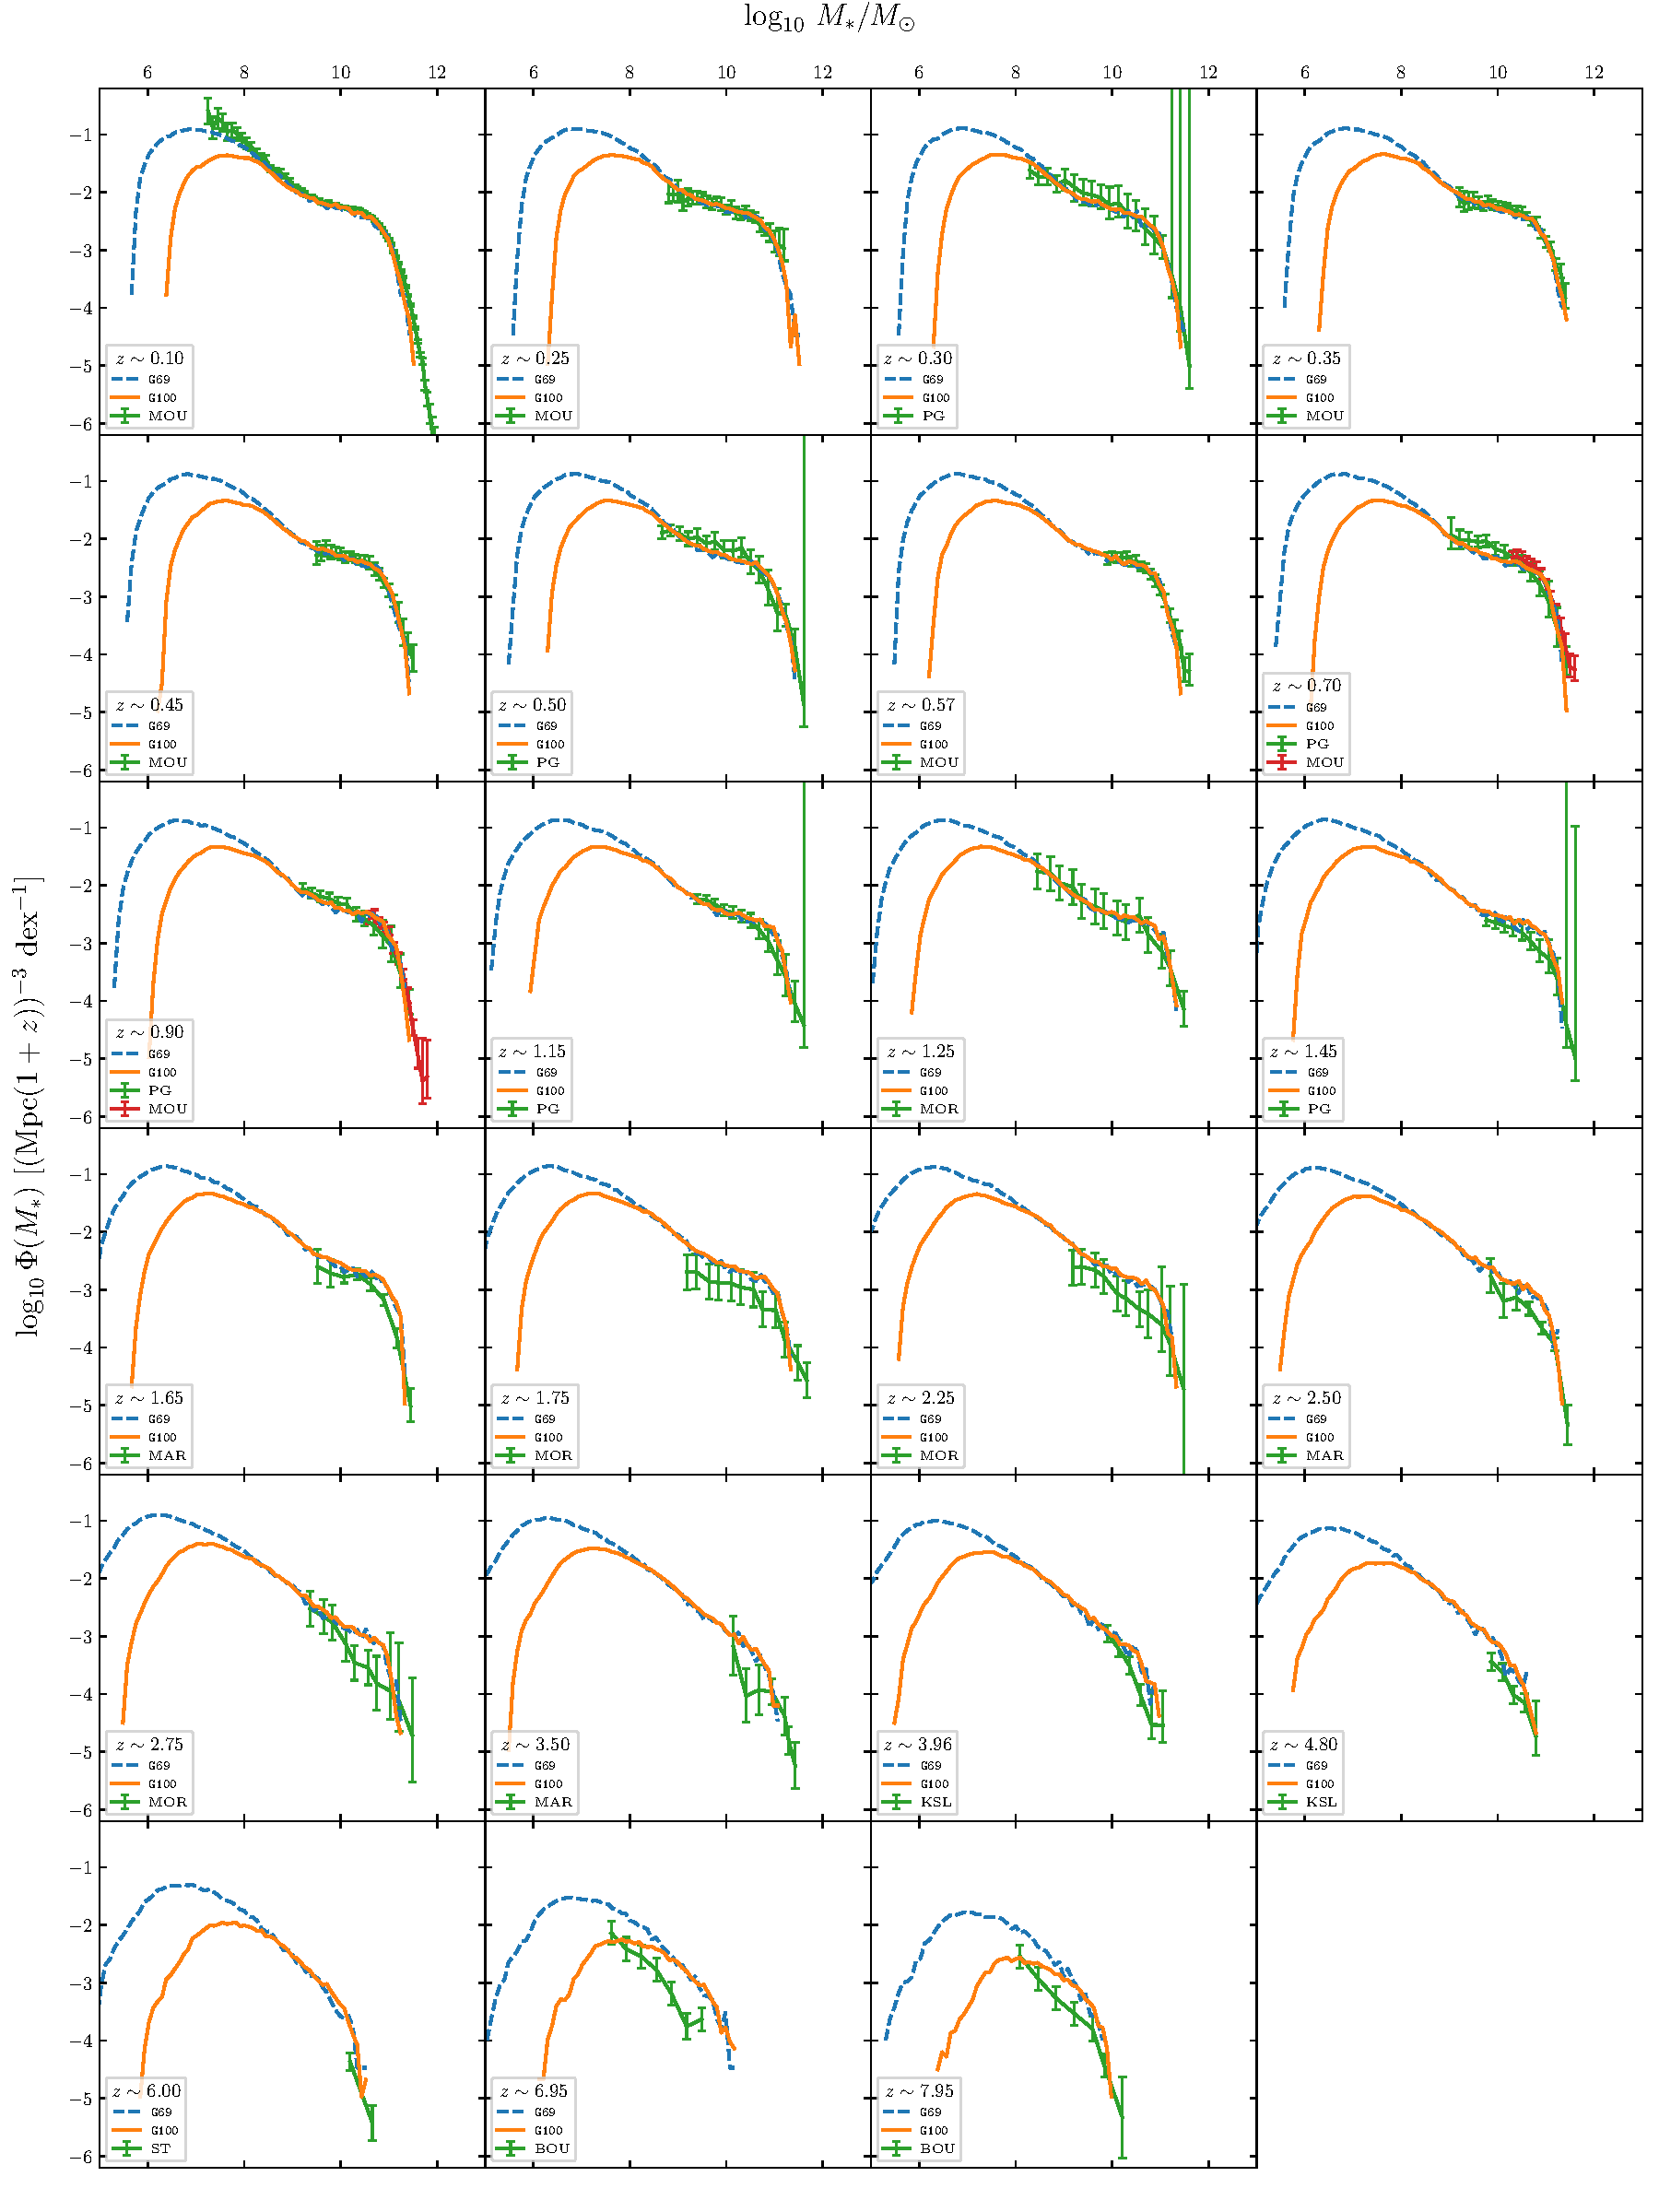
\includegraphics[width=\textwidth]{images/smf/smf_both_sims.pdf}%
	\caption{
		Obtained stellar mass functions $\Phi(M_*)$ of central galaxies for the two simulation datasets \gsmall\ and \glarge, described in \ref{chap:sim_galaxy} with boxsize of 69 and 100 Mpc, respectively, compared to observed stellar mass function.
		The abbreviations used for observational data are listed in table \ref{tab:obs_smf}.
	}%
	\label{fig:smf}
\end{figure}


















%============================================================================
\subsection{Correlation Functions}\label{chap:correlation}
%============================================================================

The obtained 2PCF $\xi(r)$ and the projected correlation function $w_p(r_p)$ at $z\sim 0$ are shown in figure \ref{fig:correlations} for both the \gsmall\ and \glarge\ simulations, and they are compared to observational results from \cite{LiWhite} and \cite{Correlation1}.

\begin{figure}[H]
	\centering
	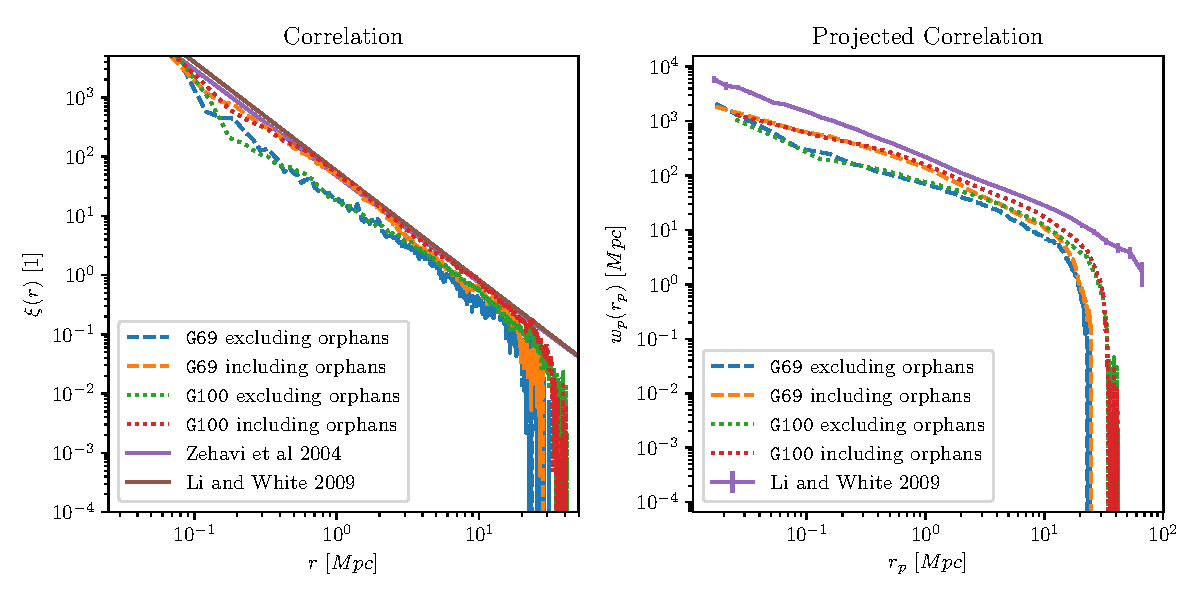
\includegraphics[width=\textwidth, keepaspectratio]{images/correlations.pdf}%
	\caption{
		The obtained 2PCF $\xi(r)$ and projected correlation function $w_p(r_p)$ for the \gsmall\ (dashed lines) and \glarge\ (dotted lines) simulations, both including and excluding orphan galaxies, compared to best power law fits of the 2PCF from \cite{LiWhite} and \cite{Correlation1} and the projected correlation function  from \cite{LiWhite} (solid lines).
	}%
	\label{fig:correlations}
\end{figure}



In all cases, including orphan galaxies produced correlation functions closer to observations.
\cite{crisis} also found that the inclusion of orphan galaxies for mass-based SHAM models may improve the clustering statistics of mock galaxy catalogues, particularly so at small scales.
The 2PCF obtained from the \glarge\ simulation even can reproduce the best power law fit from observations quite well for about two orders of magnitude of $r\sim 0.2 - 20$ Mpc.
Noticeably for both simulations the correlation functions start with very similar values regardless of whether orphan galaxies are included or not for small $r$. 
As the distance $r$ increases, so does the difference between the two cases, and starts decreasing around $r\sim 1-2 $ Mpc.
After $r\sim 10$ Mpc, the difference becomes very small.
This behaviour may be explained by considering that one would expect orphan galaxies to tend to be located within host halos, not somewhere in a void all by themselves, thus contributing to the correlations at small distances stronger than at large distances.


Any case underestimates the projected correlation function, but as for the 2PCF, the \glarge\ simulation with orphan galaxies included in the computation of the correlation comes closest.
Because $w_p$ is computed by numerically integrating the previously obtained $\xi(r)$, part of the reason why $w_p$ might be underestimated is the propagation of errors.
$w(r_p)$ is computed by integrating $\xi(r)$ from $r=r_p$ to $r\rightarrow \infty$, meaning that the underestimated $\xi(r)$ at large scales $r\gtrsim 20$ Mpc is included in the integration for every $r_p$.
Another reason might be that while technically the integration should be performed to infinity, it was truncated at half of the length of a simulation box.


The \glarge\ simulation gives better correlation functions, which might be due to the fact that a bigger volume was simulated.
A volume of 69 Mpc might just be too small to properly represent a homogeneous, isotropic chunk of the Universe.
















%%=========================================================
%\subsection{Outlook}
%%=========================================================
%
%Given that the mock galaxy catalogues in this work were created using simulations with relatively low spatial and mass resolution, the obtained correlation functions and stellar mass functions are satisfactory.
%A higher spatial resolution should improve the clustering statistics, and together with a higher mass resolution the stellar mass functions of central galaxies should also improve.
